\documentclass[12pt]{article}
\usepackage[utf8]{inputenc}
\usepackage[margin=0.9in]{geometry}
\usepackage{paralist}
\usepackage{blindtext}
\usepackage{hyperref}
\usepackage{chngcntr}
\usepackage{amsfonts,latexsym,amsthm,amssymb,amsmath,amscd,euscript}
\usepackage{enumitem}
\usepackage{caption}
\usepackage[linesnumbered]{algorithm2e}
\usepackage{algpseudocode}
\usepackage{amsmath}
\usepackage[table,xcdraw]{xcolor}
\usepackage{tikz}
\usepackage{parskip}
\usepackage{fancyhdr}

\newcommand\mycommfont[1]{\footnotesize\ttfamily\textcolor{blue}{#1}}
\SetCommentSty{mycommfont}

\usetikzlibrary{arrows.meta}

    \hypersetup{colorlinks=true,citecolor=blue,urlcolor =black,linkbordercolor={1 0 0}}

\usetikzlibrary{calc}

\renewcommand\thesubsubsection{\arabic{subsubsection}}
\newcommand{\myargfontR}{\textcolor{red}}

\newenvironment{statement}{\color[rgb]{1.00,0.00,0.50} {}}{}


\newcolumntype{M}[1]{>{\centering\arraybackslash}m{#1}}
\newcolumntype{N}{@{}m{0pt}@{}}
\algnewcommand{\algorithmicand}{\textbf{ and }}


\algnewcommand\algorithmicforeach{\textbf{for each}}
\algdef{S}[FOR]{ForEach}[1]{\algorithmicforeach\ #1\ \algorithmicdo}


\newlist{enums}{enumerate}{3}

\setlist[enums, 1]{label={(\arabic*)}, noitemsep}
\setlist[enums, 2]{label={-}, noitemsep}

\newlist{alphalist}{enumerate}{1}
\setlist[alphalist,1]{label={(\textbf{\alph*})}}


\hypersetup{
    colorlinks=true,
    linkcolor=blue,
    filecolor=magenta,
    urlcolor=black
    }

\title{ADA Assignment 2}
% \author{Anirudh S. Kumar (2021517), Aakarsh Jain (2021507)}
\author{
    \\\vspace{0em} Anirudh S. Kumar \\\vspace{-0.5em}
    \footnotesize{Roll Number - 2021517}\\\vspace{-0.5em}
    \footnotesize{IIIT - Delhi}\\\vspace{-0.5em}
    \footnotesize{\href{mailto:anirudh21517@iiitd.ac.in}{\texttt{anirudh21517@iiitd.ac.in}}}
  \and
    \\\vspace{0em} Vartika\\\vspace{-0.5em}
    \footnotesize{Roll Number - 2021571}\\\vspace{-0.5em}
    \footnotesize{IIIT - Delhi}\\\vspace{-0.5em}
    \footnotesize{\href{mailto:vartika21571@iiitd.ac.in}{\texttt{vartika21571@iiitd.ac.in}}}
    \vspace{1em}
}

\renewcommand{\footrulewidth}{0.4pt}% Default \footrulewidth is 0pt
\renewcommand{\headrulewidth}{0pt}% Default \headrulewidth is 0.4pt


\date{\today}

\begin{document}
\maketitle

\pagestyle{fancy}
\fancyhf{}
\fancyfoot[L]{Anirudh S. Kumar}
\fancyfoot[C]{\thepage}
\fancyfoot[R]{Vartika}

\section{City of Computopia}
\subsection{Problem}
\begin{statement}
    The police department in the city of Computopia has made all the streets one-way.
But the mayor of the city still claims that it is possible to legally drive from one intersection to any
other intersection.

\begin{alphalist}
    \item Formulate this problem as a graph theoretic problem and explain why it can be solved in linear time.

    \item Suppose it was found that the mayor’s claim was wrong. She has now made a weaker claim: “If
you start driving from town hall, navigating one-way streets, then no matter where you reach,
there is always a way to drive legally back to the town hall. Formulate this weaker property as
a graph theoretic problem and explain how it can be solved in linear time.
\end{alphalist}
\end{statement}


\subsection{Solution Part \textbf{(a)}}



\subsubsection{Formulation as a graph problem}
Consider the initial city as a graph $G(V, E)$ with intersections as nodes and streets as edges between them as shown in Fig \ref{fig:undirected}.

More formally, any intersection ${\textrm{\textbf{int}}}_i \in V(G)$, and $({\textrm{\textbf{int}}}_i, {\textrm{\textbf{int}}}_j) \in E(G)$ there is a road connecting intersections ${\textrm{\textbf{int}}}_i$ and ${\textrm{\textbf{int}}}_j$

\begin{figure}[ht]
\centering
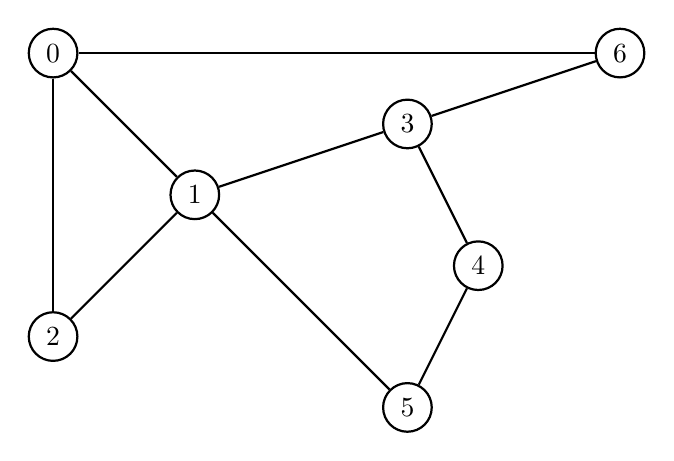
\begin{tikzpicture}[node distance={10mm}, thick, main/.style = {draw, circle}, scale=0.9]
    \node [main] (0) at (-3, 3) {0};
    \node [main] (1) at (-1, 1) {1};
    \node [main] (2) at (-3, -1) {2};
    \node [main] (3) at (2, 2) {3};
    \node [main] (4) at (3, 0) {4};
    \node [main] (5) at (2, -2) {5};
    \node [main] (6) at (5, 3) {6};

    \draw (0) to (1);
    \draw (1) to (2);
    \draw (1) to (3);
    \draw (3) to (4);
    \draw (5) to (4);
    \draw (5) to (1);
    \draw (3) to (6);
    \draw (6) to (0);
    \draw (0) to (2);

\end{tikzpicture}
\caption{two-way streets}
\label{fig:undirected}

\end{figure}

Now, the police turning all the streets to one-way means converting all the undirected edges into directed ones. as shown in Fig \ref{fig:directed}

\begin{figure}[ht]
\centering
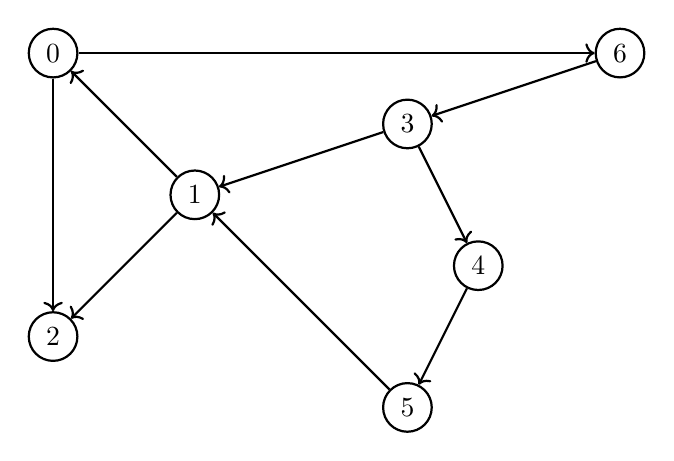
\begin{tikzpicture}[node distance={10mm}, thick, main/.style = {draw, circle}, scale=0.9]

    \node [main] (0) at (-3, 3) {0};
    \node [main] (1) at (-1, 1) {1};
    \node [main] (2) at (-3, -1) {2};
    \node [main] (3) at (2, 2) {3};
    \node [main] (4) at (3, 0) {4};
    \node [main] (5) at (2, -2) {5};
    \node [main] (6) at (5, 3) {6};


    \draw[<-] (0) to (1);
    \draw[->] (1) to (2);
    \draw[<-] (1) to (3);
    \draw[->] (3) to (4);
    \draw[<-] (5) to (4);
    \draw[->] (5) to (1);
    \draw[<-] (3) to (6);
    \draw[<-] (6) to (0);
    \draw[->] (0) to (2);

\end{tikzpicture}
\caption{One-way streets instead of 2-way}
\label{fig:directed}

\end{figure}



\subsubsection{Linear time solution}


\RestyleAlgo{ruled}

%% This is needed if you want to add comments in
%% your algorithm with \Comment

\begin{algorithm}[H]

    \SetAlgoLined \DontPrintSemicolon
    \SetKwFunction{proc}{connectedGraph}
    \SetKwProg{myproc}{procedure}{}{end}
    \SetKw{alIn}{in}
    \SetKw{alBool}{\textbf{boolean}}
    \SetKw{alF}{false}
    \SetKw{alVis}{\texttt{visited}}

    \myproc{\proc{\textcolor{red}{G}} $\rightarrow$ \alBool}{
        \tcc{Returns true if mayor's claim is true, i.e. graph is \;
        strongly connected. Otherwise, returns false}


        \alVis $\leftarrow$ boolean array of size $|V(G)|$, and initialize all to \alF \;
        pick any arbitrary node $\textrm{\textbf{int}}_i \in V(G)$ \;
        perform DFS with $\textrm{\textbf{int}}_i$ as the starting node \;
        set $vis_j$ = \textbf{true} if $\textrm{\textbf{int}}_j$ is visited in the DFS $\forall \textrm{\textbf{ int}}_j \in V(G)$\;
        \For{$vis_i$ \alIn \alVis}{
            \If{$vis_i = $ \alF}{
                \Return \textcolor{red}{false} \tcp{In case any node is not visited}
            }
        }

        \Return \textcolor{red}{true}
    }

    \caption{All intersections reachable}
    \label{alg:part1a}
\end{algorithm}

The main idea behind the algorithm is to check if the graph is strongly connected (implying that all intersections are reachable). It takes $\mathcal{O}(|V| + |E|)$ operations to perform DFS on a graph, and $\mathcal{O}(|V|)$ further operations to check if all nodes have been visited. Therefore, the overall time complexity of the algorithm is $\mathcal{O}(|V| + |E|)$, i.e. linear.

\subsection{Solution Part (b)}

\subsubsection{Formulation as a graph problem}

The formulation is the same as part (a) when converting all the streets into one-way roads.

\begin{figure}[ht]
\centering
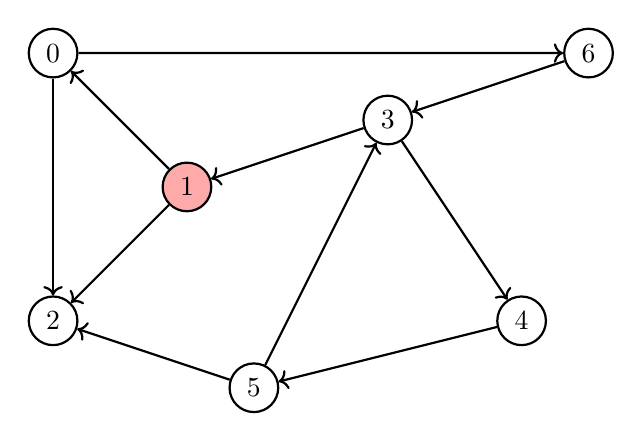
\begin{tikzpicture}[node distance={10mm}, thick, main/.style = {draw, circle}, scale=0.85]

    \node [main] (0) at (-3, 3) {0};
    \node [main, fill={rgb:red,1;white,2}] (1) at (-1, 1) {1};
    \node [main] (2) at (-3, -1) {2};
    \node [main] (3) at (2, 2) {3};
    \node [main] (4) at (4, -1) {4};
    \node [main] (5) at (0, -2) {5};
    \node [main] (6) at (5, 3) {6};


    \draw[<-] (0) to (1);
    \draw[->] (1) to (2);
    \draw[<-] (1) to (3);
    \draw[->] (3) to (4);
    \draw[<-] (5) to (4);
    \draw[->] (5) to (3);
    \draw[<-] (3) to (6);
    \draw[<-] (6) to (0);
    \draw[->] (5) to (2);
    \draw[->] (0) to (2);

\end{tikzpicture}
\caption{Cycle in a directed graph, Node 1 is the starting node or town hall}
\label{fig:cycle}

\end{figure}

\subsubsection{Linear time solution}

\begin{algorithm}[H]

    \SetAlgoLined \DontPrintSemicolon
    \SetKwFunction{proc}{connectedGraph}
    \SetKwProg{myproc}{procedure}{}{end}
    \SetArgSty{}
    \SetKw{alIn}{in}
    \SetKw{alF}{false}
    \SetKw{alVis}{\texttt{visited}}

    \myproc{\proc{\textcolor{red}{G}} $\rightarrow$ boolean}{
        \tcc{Returns true if there is a path from town hall to itself, false otherwise}


        Convert $G$ into a condensation graph using Kosaraju's algorithm. \;
        Let the new graph be $C(V, E)$ \;
        Let $U \in V(C)$ be of the form $U = \{ u_1, u_2, \dots, u_k \}$ where $u_i \in V(G)$ \;

        Let $T \in V(C)$ be the condensation node which contains the town-hall \;
        \For{$U \in V(C)$}{
            \For{$u \in U$}{
                set label($u) = U$ \;
            }
        }

        \For{$(u_1, u_2) \in E(G)$}{
            \If{ label($u_1$) = $T$ $\wedge$ label($u_2$) $\neq$ $T$}{
                \Return \textcolor{red}{false} \;
            }
        }


        \Return \textcolor{red}{true}
    }

    \caption{All intersections reachable}
    \label{alg:part1b}
\end{algorithm}

Kosaraju's algorithm takes $\mathcal{O}(|V| + |E|)$ to form the condensation graph, and then further $\mathcal{O}(|E|)$ operations are performed to check all the edges. Therefore, the overall time complexity of the algorithm is $\mathcal{O}(|V| + |E|)$, i.e. linear.

\pagebreak

\section{Smallest weight in a cycle}

\subsection{Problem}

\begin{statement}
    Given an edge-weighted connected undirected graph $G = (V, E)$ with $n + 20$ edges.
Design an algorithm that runs in $\mathcal{O}(n)$-time and outputs an edge with the smallest weight contained in a cycle of $G$. You must give a justification for why your algorithm works correctly
\end{statement}
% \begin{figure}[ht]
% \centering
% \begin{tikzpicture}[node distance={10mm}, thick, main/.style = {draw, circle}]
%     \node [main] (0) at (-3, 3) {0};
%     \node [main] (1) at (-1, 1) {1};
%     \node [main] (2) at (-4, 0) {2};
%     \node [main] (3) at (2, 2) {3};
%     \node [main] (4) at (5, 1) {4};
%     \node [main] (5) at (2, 0) {5};
%     \node [main] (6) at (5, 3) {6};

%     \draw (0) -- node[midway, above right] {\textcolor{red}{10}}  (1) ;
%     \draw (1) -- node[midway, above left ] {\textcolor{red}{10}} (3);
%     \draw (3) -- node[midway, above right] {\textcolor{red}{6}} (4);
%     \draw (5) -- node[midway, above left ] {\textcolor{red}{3}} (4);
%     \draw (3) -- node[midway, above left ] {\textcolor{red}{4}} (6);
%     \draw (6) -- node[midway, above      ] {\textcolor{red}{7}} (0);
%     \draw (0) -- node[midway,       left ] {\textcolor{red}{1}} (2);

% \end{tikzpicture}
% \caption{Weighted graph}
% \label{fig:weighted_graph}

% \end{figure}

\subsection{Solution}

\subsubsection{Linear Time Algorithm}

\begin{algorithm}[H]

    \SetAlgoLined \DontPrintSemicolon
    \SetKwFunction{proc}{smallestCycleEdge}
    \SetKwProg{myproc}{procedure}{}{end}

    \SetKwFunction{args}{parentDFS}
    \SetArgSty{}
    \SetKw{alIn}{in}
    \SetKw{alInt}{int}
    \SetKw{alMinW}{$min_w$}
    \SetKw{alAdj}{Adj($u$)}
    \SetKw{alVis}{\texttt{visited}}

    \tcp{global variables}
    \alMinW $\leftarrow \infty$   \;
    \alVis $\leftarrow$ boolean array of size $|V(G)|$, and initialize all to false \;
    $\textrm{curr}_{\textrm{min}}\leftarrow \infty$ \;

    \;

    \myproc{\args{v}}{
        set $vis_v = $ true \;\;

        \For{$p$ in \textbf{Adj($v$)}}{
            \If{$vis_p = $ \textbf{false}}{
                parent(w) = v \;
                $\textrm{curr}_{\textrm{min}} = \textrm{\textbf{min}}(\textrm{curr}_{\textrm{min}}, (p, v))$ \tcp{ (u,v) is the weight of the }
                Run \args{p} \;
            }
            \;
            \If {$vis_p = $ \textbf{true} $\wedge$ parent(p) $\neq v$ }{
                $min_w = \textrm{\textbf{min}}(min_w$,  $\textrm{curr}_{\textrm{min}})$ \;
                $\textrm{curr}_{\textrm{min}} \leftarrow \infty$ \;
            }
        }
    }

    \;


    \myproc{\proc{\textcolor{red}{G}} $\rightarrow$ \alInt}{
        \tcc{Returns smallest weight contained in a cycle of $G$. \;
        Returns $\infty$ if there is no cycle in $G$}

        consider any arbitrary vertex $u$ as the starting node \;
        Run \args{u} \;


        \Return $min_w$
    }

    \caption{Smallest weight contained in a cycle of G}
    \label{alg:part2}
\end{algorithm}

The main idea behind Algorithm \ref{alg:part2} is to keep track of current minimum edge, and then update the global minimum edge when it detects a loop.


\subsubsection{Correctness Proof}
\textbf{Assumption}: A cycle contains 3 or more vertices, i.e. no self-loops and edge being considered as loop.

Any undirected connected graph $G = (V, E)$ can be cyclic or acyclic.

\textbf{Case 1: Acyclic} - In this case, it will never be possible for a vertex $v \in V(G)$ to be both visited and have its parent not be the current node, i.e. $u \in V(G)$.

\begin{enumerate}
    \item If $v$ is not visited, then its parent will be set to $u$ and marked visited.
    \item If $v$ is visited, its parent must be $u$. Assume by contradiction that $v$ is visited, and its parent is $w \in V(G)$. This implies a cycle since we know a path from $u$ to $w$ (the graph is known to be connected). We have just encountered the edge $(u, v) \because v \in$ Adj($u$), and parent($v$) = $w$, so there is also an edge $(v, w)$, thus completing the cycle.
\end{enumerate}

Thus, the value of $min_w$ remains $\infty$ implying there is no cycle in the graph and therefore no minimum edge

\begin{figure}[ht]
\centering
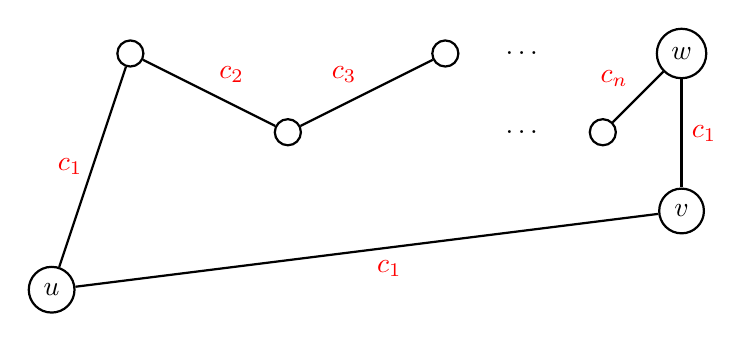
\begin{tikzpicture}[node distance={10mm}, thick, main/.style = {draw, circle}]
    \node [main] (0) at (-3, 3) {};
    \node [main] (1) at (-1, 2) {};
    \node [main] (2) at (-4, 0) {$u$};
    \node [main] (3) at (1, 3) {};
    \node [main] (6) at (3, 2) {};
    \node [main] (4) at (4, 1) {$v$};
    \node [main] (5) at (4, 3) {$w$};
    \node at (2, 3) {$\dots$};
    \node at (2, 2) {$\dots$};


    \draw (0) -- node[midway, above right] {\textcolor{red}{$c_2$}}  (1) ;
    \draw (1) -- node[midway, above left ] {\textcolor{red}{$c_3$}} (3);
    \draw (0) -- node[midway,       left ] {\textcolor{red}{$c_1$}} (2);
    \draw (6) -- node[midway, above left ] {\textcolor{red}{$c_n$}} (5);
    \draw (5) -- node[midway,       right ] {\textcolor{red}{$c_1$}} (4);
    \draw (2) -- node[midway, below right ] {\textcolor{red}{$c_1$}} (4);

\end{tikzpicture}
\caption{Cycle condition}
\label{fig:contradiction}

\end{figure}



\textbf{Case 2: Cyclic} If there is a cycle, there will always be a case where $v$ is visited and parent$(v) \neq u$. There will always be a node $u$ with a path from it to itself, as shown in Fig \ref{fig:cycle}. We always maintain the minimum edge along the cycle and update it with $min_w$ when we reach the cycle's starting point, giving us the smallest edge weight in all cycles of $G$.

Also, the fact that we only need to call \args{} once stems from the fact that the graph is connected, and the DFS Tree of any one node will contain all the graph nodes.

\subsubsection{Time Complexity}

% The algorithm's time complexity is $\mathcal{O}(|V| + |E|)$ since DFS will only visit the graph nodes once. Once we visit a vertex, we will only visit it at most once, which will

In \args{u}, we visit a node at max 2 times, once when it is marked visited and once when we go to check if it is visited and the parent is not $u$. Therefore, time complexity of the algorithm is linear, i.e. $\mathcal{O}(|V| + |E|)$


\pagebreak

\section{Probability of reaching sink}

\subsection{Problem}

\begin{statement}
    Suppose that $G$ be a directed acyclic graph with the following features
    \begin{itemize}
        \item $G$ has a single source $s$ and several sinks $t_1, \dots , t_k$
        \item Each edge $(v \rightarrow w)$ (i.e. an edge directed from $v$ to $w$) has an associated weight $Pr(v \rightarrow w)$ between 0 and 1.
        \item For each non-sink vertex $v$, the total weight of all the edges leaving $v$ is $$\sum_{(v \rightarrow w) \in E} Pr(v \rightarrow w) = 1$$
    \end{itemize}

The weights $Pr(v \rightarrow w)$ define a random walk in $G$ from the source $s$ to some sink $t_i$
; after reaching any non-sink vertex $v$, the walk follows the edge $v \rightarrow w$ with probability $Pr(v \rightarrow w)$.

All the probabilities are mutually independent. Describe and analyze an algorithm to compute the
probability that this random walk reaches sink $t_i$
for every $i \in {1, \dots , k}$. You can assume that an
arithmetic operation takes $\mathcal{O}(1)$ time.
\end{statement}

\begin{figure}[ht]
\centering
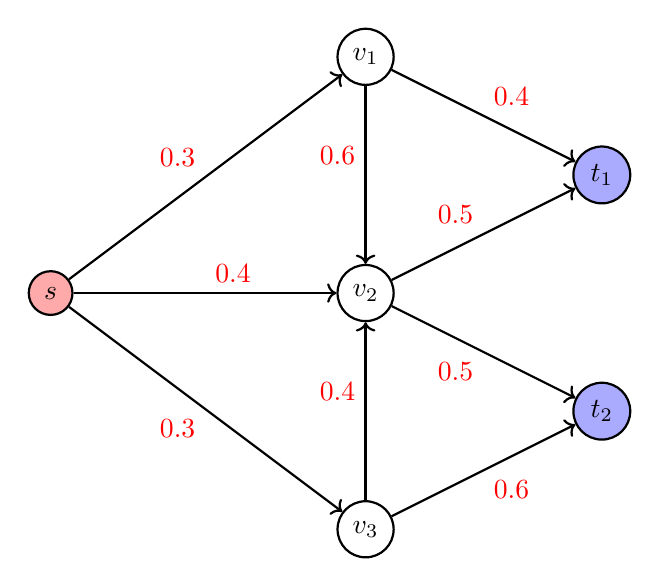
\begin{tikzpicture}[node distance={10mm}, thick, main/.style = {draw, circle}]
    \node [main] (0) at (0, 0) {$v_2$};
    \node [main] (1) at (0, 3) {$v_1$};
    \node [main, fill={rgb:blue,1;white,2}] (2) at (3, 1.5) {$t_1$};
    \node [main] (3) at (0, -3) {$v_3$};
    \node [main, fill={rgb:blue,1;white,2}] (4) at (3, -1.5) {$t_2$};
    \node [main, fill={rgb:red,1;white,2}] (5) at (-4, 0) {$s$};


    \draw[->] (5) -- node[midway, above left ] {\textcolor{red}{0.3}} (1);
    \draw[->] (5) -- node[midway, above right] {\textcolor{red}{0.4}} (0);
    \draw[->] (5) -- node[midway, below left ] {\textcolor{red}{0.3}} (3);
    \draw[->] (3) -- node[midway, above left ] {\textcolor{red}{0.4}} (0);
    \draw[->] (1) -- node[midway, above left ] {\textcolor{red}{0.6}} (0);
    \draw[->] (1) -- node[midway, above right] {\textcolor{red}{0.4}} (2);
    \draw[->] (0) -- node[midway, above left ] {\textcolor{red}{0.5}} (2);
    \draw[->] (3) -- node[midway, below right] {\textcolor{red}{0.6}} (4);
    \draw[->] (0) -- node[midway, below left ] {\textcolor{red}{0.5}} (4);

\end{tikzpicture}
\caption{An Example Network Flow Graph. Probabilities are mentioned on every edge. The source vertex is coloured red, and sinks are coloured blue}
\label{fig:network_flow}
\end{figure}


\subsection{Solution}

\subsubsection{Sub-problem}

Probability of reaching the sink $t_i$ from vertex $v$, denoted as $P(v, t_i)$.

\subsubsection{Recurrence Relation}

\textbf{Base Case:} $P(t_i, t_i) = 1$, and $P(v, t_i) = 0$  $ \forall v \neq t_i$


\textbf{Recurrence Relation :-}

$$P(v, t_i) = \sum_{(v \rightarrow w) \in E} Pr(v \rightarrow w) \times P(w, t_i)$$

In other words, the probability of reaching from $v$ to $t_i$ is the sum of the probability of going from $v$ to $w$ times the probability of reaching from $w$ to $t_i$

\subsubsection{Subproblem which gives solution}

$P(s, t_i)$, which gives the probability of reaching sink $t_i$ from $s$

\subsubsection{Algorithm}

\begin{algorithm}[H]

    \SetAlgoLined \DontPrintSemicolon
    \SetKwFunction{proc}{pSinks}
    \SetKwProg{myproc}{procedure}{}{end}

    \SetKwFunction{arg}{computeProb}
    \SetKwProg{computeProbs}{procedure}{}{end}

    \SetArgSty{}
    \SetKw{alArr}{\textbf{array}}


    \computeProbs{\arg{$G, u, v, P$}}{
        \If {$u = v = t_i$}{
            \Return \;
        }
        \texttt{curr\textunderscore val} $\leftarrow$ 0 \tcp{for storing current value of $P(u, v)$}
        \For{$w \in$ \textbf{Adj($u$)}}{
            \If{$P(w, v) = -1$}{
                Run \arg{$G, w, v, P$} \;
            }
            \texttt{curr\textunderscore val+=} $Pr(u \rightarrow w) \times P(w, v)$ \;
        }
        $P(u, v) = $ \texttt{curr\textunderscore val}

    }



    \;

    \myproc{\proc{\textcolor{red}{G}} $\rightarrow$ \alArr}{
        \tcc{Returns an array \textbf{pathProb} where \textbf{pathProb[i]} is probability of reaching sink $t_i$ from source $s$.
        Assuming the graph has $n$ sinks $t_1, t_2, \dots, t_n$}

        $P$ $\leftarrow$ 2-D array to store value of $P(u, v)$  $ \forall u,v \in V(G)$ \;
        \texttt{pathProb} $\leftarrow$ array to store value of $P(s, t_i)$ \;
        Initialize all values in \texttt{pathProb} to 0 and in $P$ to -1 \;

        \;

        \For{$i = 1$ \KwTo n }{
            $P(t_i, t_i) = 1$   \;
        }

        \For{$i$ = 1 \KwTo n }{
            Run \texttt{computeProb($G, s, t_i, P$)} \;
            \texttt{pathProbs[i]} = $P(s, t_i)$ \;
        }

        \Return \texttt{pathProbs} \;


    }

    \caption{Probability of reaching sinks}
    \label{alg:part3}
\end{algorithm}

\pagebreak

\subsubsection{Time Complexity}

For every sink $t_i$, We will traverse through the entire graph in a DFS-type manner and then backtrack to fill the values of the edges already visited, as can be seen in the recursive nature of the algorithm. Therefore, the time complexity for finding $P(s, t_i)$ is $\mathcal{O}(|V| + |E|)$

If there are $n$ such sinks, then the algorithm will be repeated $n$ times for each sink. Therefore, total time complexity of the algorithm is $\mathcal{O}(n(|V| + |E|))$




\end{document}
